\documentclass[11pt]{article}
\renewcommand{\baselinestretch}{1.05}
\usepackage{amsmath,amsthm,verbatim,amssymb,amsfonts,amscd, graphicx}
\usepackage{blindtext}

\usepackage{caption}
\usepackage{enumitem}

%Additional Packages
\usepackage{enumitem}
\usepackage{graphics}
\usepackage{float}
\graphicspath{ {images/} }
%\usepackage[framed]{mcode}
\usepackage{hyperref}
\hypersetup{
	colorlinks=true,
	linkcolor=blue,
	filecolor=magenta,      
	urlcolor=cyan,
}

\topmargin0.0cm
\headheight0.0cm
\headsep0.0cm
\oddsidemargin0.0cm
\textheight23.0cm
\textwidth16.5cm
\footskip1.0cm
\theoremstyle{plain}
\newtheorem{theorem}{Theorem}
\newtheorem{corollary}{Corollary}
\newtheorem{lemma}{Lemma}
\newtheorem{proposition}{Proposition}
\newtheorem*{surfacecor}{Corollary 1}
\newtheorem{conjecture}{Conjecture} 
\newtheorem{question}{Question} 
\theoremstyle{definition}
\newtheorem{definition}{Definition}

\usepackage{indentfirst}
%\renewcommand{\thesubsubsection}{\thesubsection.\alph{subsection}}

\newcommand{\floor}[1]{\lfloor #1 \rfloor}

%SETUP PSUEDOCODE
\usepackage{tcolorbox}


%SETUP AtxMEGA128A1U
\usepackage{listings}

\usepackage{xcolor}
\definecolor{bluekeywords}{rgb}{0.13,0.13,1}
\definecolor{greencomments}{rgb}{0,0.5,0}
\definecolor{turqusnumbers}{rgb}{0.17,0.57,0.69}
\definecolor{redstrings}{rgb}{0.5,0,0}

\lstdefinelanguage{atxmega128a1u}{
	morekeywords={include, ,org, def, rjmp, CSEG, db, equ, DSEG, ldi, lds, sts,  breq, brne, and, cp, cpi, push, pop, ret, reti, sbrs, call, lpm, mov, jmp},
	keywordstyle=\color{bluekeywords},
	sensitive=false,
	morecomment=[l][\color{greencomments}]{;},
	morecomment=[s][\color{greencomments}]{{/*}{*/}},
	morestring=[b]",
	stringstyle=\color{redstrings}
}

\lstnewenvironment{asmlisting}{
	\lstset{
		frame=single,
		language=atxmega128a1u,
		basicstyle=\ttfamily,
		breaklines=true,
		columns=fullflexible
	}
}
{}
%
% START OF DOCUMENT
%
\begin{document}
\captionsetup[figure]{labelfont=bf} 

\title{Lab 4}
\author{\textbf{Michael Arboleda}\\Lab Section: 7F34}
\maketitle
%
% PRELAB QUESTIONS
%
\section*{b. Answers to all pre-lab questions}

\textbf{\textcolor{red}{Part A Question}:} Determine which pins on PORTD are used for USARTD0?\\
\textbf{Ans: } Pin 2 and Pin 3 are used for USARTD0
\begin{enumerate}[label={\arabic*)},font={\color{red}\bfseries}]
	%
	%1
	%
	\item What is the difference between serial and parallel communication?
	\\[0.8ex]
	\textbf{ANS: } Serial using one pin, while parallel uses multiple pins
	%
	%2
	%
	\item What is the difference between synchronous and asynchronous communication?
	\\[0.8ex]
	\textbf{ANS: } Synchronous communication means the transmitter and receiver are on the same clock. Asynchronous communication use Start and Stop bits and Baud rate to determine the speed and also uses parity bit for error checking 
	%
	%3
	%
	\item List the XMEGA’s USART registers used in your programs and briefly describe their functions.
	\\[0.8ex]
	\textbf{ANS: }\\
	\textbf{\textcolor{blue}{DATA:}} This contains the data that was transmitted/received 
	\\
	\textbf{\textcolor{blue}{STATUS:}} Contains flags like Receive Complete Interrupt Flag, Transfer Complete Interrupt Flag, and Data Register Empty Interrupt Flag. 
	\\
	\textbf{\textcolor{blue}{CTRLC:}} Used to set up serial mode, width of data, parity, and number of stop bits
	\\
	\textbf{\textcolor{blue}{CTRLB:}} Used to enable properties of USARTD0 such as receive and transmit  
	\\
	\textbf{\textcolor{blue}{CTRLA:}}
	Used to set up the level of the different types of interrupts for USARTD0
	\\
	\textbf{\textcolor{blue}{BAUDCTRLB:}} Sets the BSCALE in the 4 upper bits [7:4] and sets bit 11:8 for BSEL in 4 lower bits [3:0]
	\\
	\textbf{\textcolor{blue}{BAUDCTRLA:}} Sets bit 7:0 for BSEL in the respective order
	
	%
	%4
	%
	\item What is the maximum possible baud you can use for asynchronous communication if your board runs at 32 MHz? Support your answer with the values you	would place in any special registers that are needed.
	\\[0.8ex]
	\textbf{ANS: } Setting BAUD control A and B (BAUDCTRLA and BAUDCTRLB) to 0b00000000 would make the Baud rate 2Mb per second
\end{enumerate}
%
% PROBLEMS ENCOUNTERED
%
\section*{c. Problems Encountered} 
My logic for ignoring invalid chars in part D was incorrect. I forgot to pop registers I had pushed.  
%
% FUTURE WORK
%
\section*{d. Future Work/Applications}
In this lab only one configuration for serial. It would be useful to try and make working programs for different serial configuration. I could also combine switches so i could set up the ascii value on the switches and transmit the corresponding character.    
%
% SCHEMATICS
%
\section*{e. Schematics}
N/A
%
% PSEUDOCODE
%
\newpage
\section*{g. Pseudocode/Flowcharts}
%
% PSEUDOCODE PART B
%
\textbf{\textcolor{blue}{Pseudocode for lab4\textunderscore serial.asm:}}
\begin{tcolorbox}
\begin{verbatim}
MAIN:
    * Equate numbers
    * Set registers to hold constants
    * Call Change_CLK_32HZ subroutine
    
WHILE(TRUE){}
END


SUBROUTINE USART_INIT
    * Set Pins to Transmit and Recieve
    * Set up USART controls 
    * Set up Baud Rate controls
    * Return to program

SUBROUTINE OUT_CHAR
    While(Transmitting){}
    * Transmit USART Data in R1
    * Return to program    	
	
SUBROUTINE OUT_STRING
    While(Z-point does not equal NULL){
        * increment Z-pointer
        * Store Z-pointer Data in R1 
    	* Call OUT_CHAR
    }
    * Return to program      

SUBROUTINE IN_CHAR
    While(Transmitting){}
    * Store USART Data into R1
    * Return to program 

SUBROUTINE Change_CLK_32HZ
    * Enable the new oscillator

    WHILE(OSC FLAG not set){}

    * Write the “IOREG” signature to the CPU_CCP reg
    * Select the new clock source in the CLK_CTRL reg
    * Return to program
\end{verbatim}
\end{tcolorbox}
%
% PSEUDOCODE PART C
%
\newpage
\textbf{\textcolor{blue}{Pseudocode for lab4\textunderscore serial\textunderscore baud\textunderscore test.asm:}}
\begin{tcolorbox}
\begin{verbatim}
MAIN:
    * Equate numbers
    * Set registers to hold constants
    * Call Change_CLK_32HZ subroutine
    * LOAD 'U' into R1
WHILE(TRUE){}
    * Call OUT_CHAR
END

SUBROUTINE USART_INIT
    * Set Pins to Transmit and Recieve
    * Set up USART controls 
    * Set up Baud Rate controls
    * Return to program

SUBROUTINE OUT_CHAR
    While(Transmitting){}
    * Transmit USART Data in R1
    * Return to program
\end{verbatim}
\end{tcolorbox}	
%
% PSEUDOCODE PART D
%
\newpage
\textbf{\textcolor{blue}{Pseudocode for lab4\textunderscore serial\textunderscore menu.asm:}}
\begin{tcolorbox}
\begin{verbatim}
MAIN:
    * Equate numbers
    * Set registers to hold constants
    * Call Change_CLK_32HZ subroutine
    * Call Display_Menu
WHILE(TRUE){}
    * Call IN_CHAR
    * Call Z_POINTER_LOGIC
    if(Valid Choice){
        * Display Menu
    }
END

SUBROUTINE Z_POINTER_LOGIC
	* Set Valid choice as true
    IF(Data = 1){
        * Point Z-Pointer to Food string
    }
    ELSE IF(Data = 2){
        * Point Z-Pointer to Quote string
    }
    ELSE IF(Data = 3){
        * Point Z-Pointer to Movie string
    }
    ELSE IF(Data = 4){
        * Point Z-Pointer to UF Course string
    }
    ELSE IF(Data = 5){
        * Point Z-Pointer to Hobby string
    }
    ELSE IF(Data = 6){
        * Return to program
    }
    ELSE IF(Data = D or Data = d){
    	WHILE(TRUE){}
    }
    ELSE{
        * Set Valid choice as false
        * Return to program
    }
    * Call OUT_STRING
    * Return to program
\end{verbatim}
\end{tcolorbox}   
\begin{tcolorbox}
\begin{verbatim}    
SUBROUTINE Display_Menu 
     * Point Z-Pointer to Menu string
     * Call OUT_STRING
     * Return to program
     
        
SUBROUTINE USART_INIT
    * Set Pins to Transmit and Recieve
    * Set up USART controls 
    * Set up Baud Rate controls
    * Return to program


SUBROUTINE OUT_CHAR
    While(Transmitting){}
    * Transmit USART Data in R1
    * Return to program    	


SUBROUTINE OUT_STRING
    While(Z-point does not equal NULL){
        * increment Z-pointer
        * Store Z-pointer Data in R1 
        * Call OUT_CHAR
    }
    * Return to program      


SUBROUTINE IN_CHAR
    While(Transmitting){}
    * Store USART Data into R1
    * Return to program 


SUBROUTINE Change_CLK_32HZ
    * Enable the new oscillator

    WHILE(OSC FLAG not set){}

    * Write the “IOREG” signature to the CPU_CCP reg
    * Select the new clock source in the CLK_CTRL reg
    * Return to program         
\end{verbatim}
\end{tcolorbox}
%
% PSEUDOCODE PART E
%
\newpage
\textbf{\textcolor{blue}{Pseudocode for lab4\textunderscore serial\textunderscore int.asm:}}
\begin{tcolorbox}
\begin{verbatim}
MAIN:
    * Equate numbers
    * Set registers to hold constants
    * Call Change_CLK_32HZ subroutine
	* Call Counter_INIT subroutine
	* Call USART_INIT subroutine

WHILE(TRUE){}
	if(Counter = 0){
	    * Toggle LED ON/OFF
	}	
END

SUBROUTINE Counter_INIT
    * Set TOP(PER) of counter
    * Set Clock Prescalar
    * Return to program  

ISR USART_ISR
    * STORE USART DATA in R1
    * Clear interrupt flag
    * Call OUT_CHAR
    * Return
    
SUBROUTINE USART_INIT
    * Set Pins to Transmit and Recieve
    * Set up USART controls 
    * Set up Baud Rate controls
    * Return to program
    
SUBROUTINE OUT_CHAR
    While(Transmitting){}
    * Transmit USART Data in R1
    * Return to program     
    
SUBROUTINE Change_CLK_32HZ
    * Enable the new oscillator

    WHILE(OSC FLAG not set){}

    * Write the “IOREG” signature to the CPU_CCP reg
    * Select the new clock source in the CLK_CTRL reg
    * Return to program    
\end{verbatim}
\end{tcolorbox}










\newpage
\section*{h. Program Code}
\textbf{\textcolor{blue}{Code for lab4\textunderscore serial.asm:}}
\lstinputlisting[language=atxmega128a1u, frame=single]{lab4_serial.asm}
\newpage
\textbf{\textcolor{blue}{Code for lab4\textunderscore serial\textunderscore baud\textunderscore test.asm:}}
\lstinputlisting[language=atxmega128a1u, frame=single]{ lab4_serial_baud_test.asm}
\newpage
\textbf{\textcolor{blue}{Code for lab4\textunderscore serial\textunderscore menu.asm:}}
\lstinputlisting[language=atxmega128a1u, frame=single]{lab4_serial_menu.asm}
\newpage
\textbf{\textcolor{blue}{Code for lab4\textunderscore serial\textunderscore int.asm:}}
\lstinputlisting[language=atxmega128a1u, frame=single]{lab4_serial_int.asm}

\newpage
\section*{i. Appendix}
\begin{figure}[H]
	\centering
	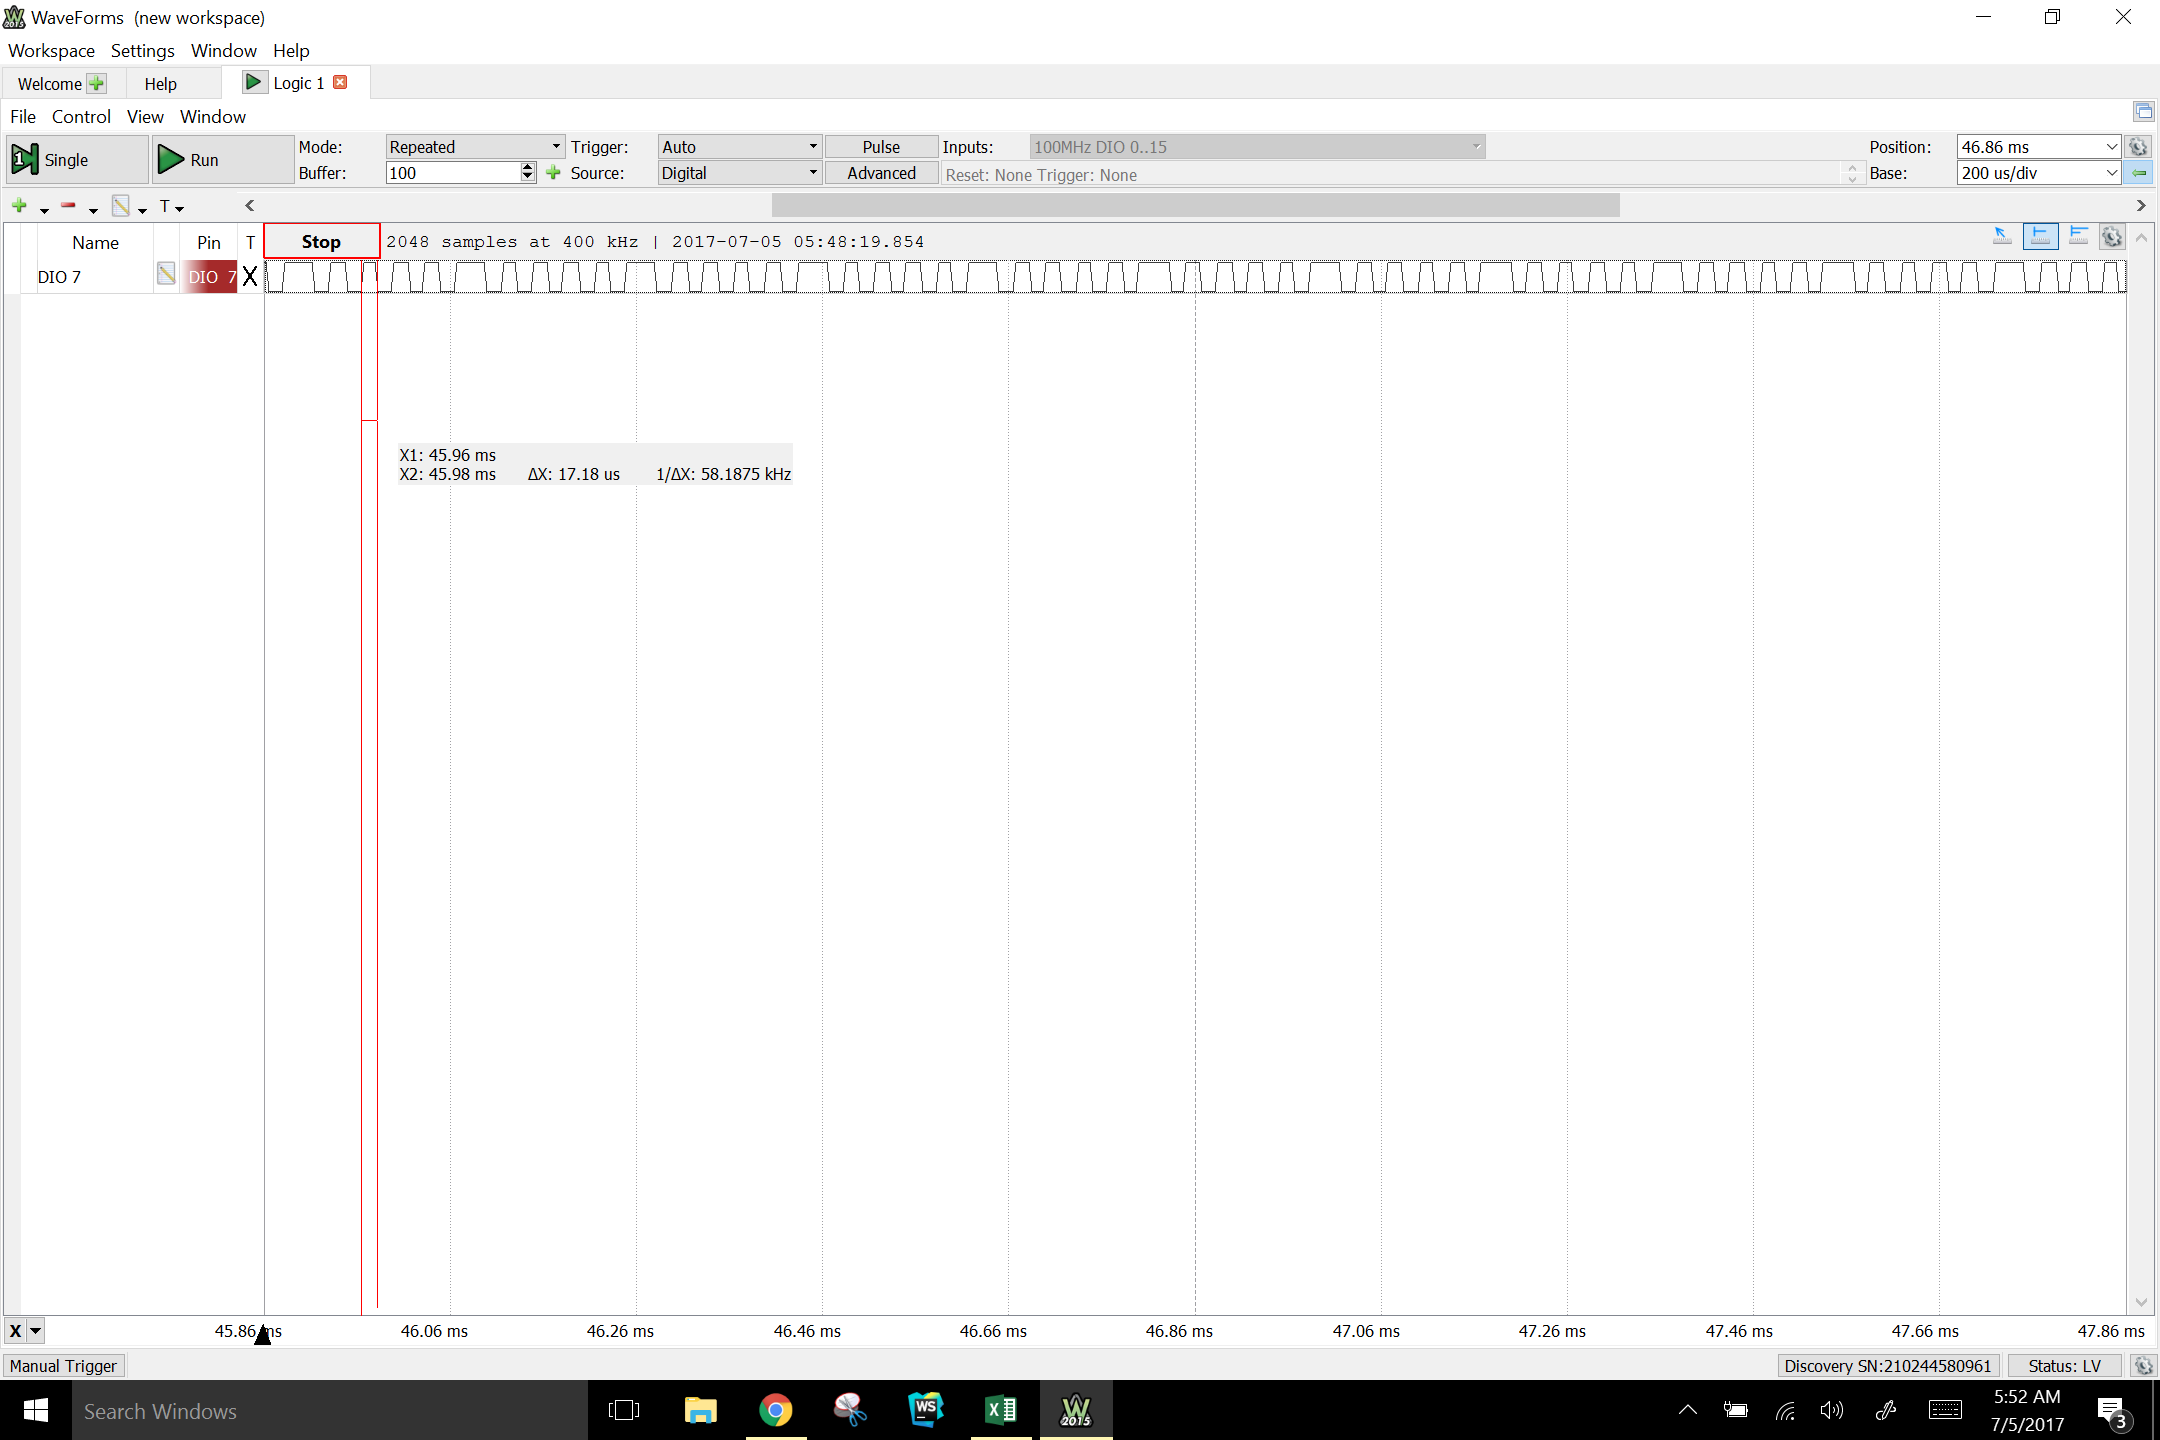
\includegraphics[width=\textwidth]{4C1}
	\label{fig:c}
	\caption{Data for one bit}
\end{figure}
Using $\dfrac{1}{57600 Hz} = 17.361 \mu S$ we see that one bit should be around for 17.361 micro seconds. The screen shot shows a frequency of 58187.5HZ and 17.18 micro seconds for one bit. This is close to the theoretical. 
\begin{figure}[H]
	\centering
	\includegraphics[width=\textwidth]{4c2}
	\label{fig:c}
	\caption{Data for entire serial transmission}
\end{figure}
Since there are 11 bits, 1 for start, 8 for data, 1 for parity and 1 for stop, the time for the serial transmission should be $11 * 17.361 \mu S = 190.971 \mu S$. According to the screen shot it takes 182.5 $\mu$S, which is close to the theoretical
\end{document}